\subsection{lead compensation}
$$
G_c(s) = K_c\dfrac{s + \dfrac{1}{T}}{s+\dfrac{1}{\alpha T}}, \quad 0 < \alpha < 1
$$
$$
G_c(s) = K_c \alpha \dfrac{Ts + 1}{\alpha T s + 1}
$$
Define:
$$K_c\alpha = K$$
then:
$$
G_c(s) = K \dfrac{Ts + 1}{\alpha T s + 1}
$$
The open-loop transfer function of the compensated system is:
$$
G_c(s)G(s) = G_c(s) = K \dfrac{Ts + 1}{\alpha T s + 1} G(s)
= G_c(s) = \dfrac{Ts + 1}{\alpha T s + 1}KG(s) = G_c(s) = \dfrac{Ts + 1}{\alpha T s + 1}G_1(s)
$$
Where:
$$
KG(s)= G_1(s)
$$
Steady state error must be less than $0.05\%$
$$
e_{ss} = \lim_{s\to 0} = \dfrac{1}{1+G_1(0)} = 0.05 \to 0.05 + 0.05G_1(0) = 1 \to 0.95 = 0.05G_1(0) \to G_1(0) = 19
$$
$$
\lim_{s\to 0} G(s) = \lim_{s\to 0} \dfrac{50(s+0.5)}{(s+1)(s+1.5)^{3}(s+2)} = \dfrac{50\times0.5}{1\times1.5^3\times2} = 3.7037 \xrightarrow[G_1 = KG]{G_1(0) = 19} K = 5.1300
$$




The amplitude ratio:
$$
\left\vert G(j\omega) \right\vert = \dfrac{50\sqrt{\omega^2+0.5^2}}{\sqrt{\omega^2+1^2}\times(\sqrt{\omega^2 + 1.5^2})^3\times\sqrt{\omega^2 + 2^2}}
$$
Gain Crossover frequency:
$$
\left\vert G(j\omega_g) \right\vert = 1
$$
\newline
$$
\dfrac{50\sqrt{\omega_g^2+0.5^2}}{\sqrt{\omega_g^2+1^2}\times(\sqrt{\omega_g^2 + 1.5^2})^3\times\sqrt{\omega_g^2 + 2^2}} = 1
$$
$$
{2500({\omega_g^2+0.25}}) = 
{({\omega_g^2+1})({\omega_g^2 + 2.25})^3({\omega_g^2 + 4}})
$$
This equation solved with MATLAB and code has attacked (Q1\_a.m).
$$
\omega_g = 2.037
$$

The phase angle:

$$
\angle G(j\omega) = 0^{\circ} + \tan^{-1}\dfrac{\omega}{0.5} - \tan^{-1}\dfrac{\omega}{1} - 3\tan^{-1}\dfrac{\omega}{1.5} - \tan^{-1}\dfrac{\omega}{2}
$$

$$
\angle G(j\omega_g) = \tan^{-1}\dfrac{2.037}{0.5} - \tan^{-1}\dfrac{2.037}{1} - 3\tan^{-1}\dfrac{2.037}{1.5} - \tan^{-1}\dfrac{2.037}{2} = -3.3871_{rad} = -194.0702^{\circ}
$$
Phase margin:
$$
\gamma = 180 + \angle G(j\omega_g) = 180 - 194.0702 = -14.0702
$$
Now we check above calculation with MATLAB margin function.
\begin{figure}[H]
	\caption{Bode digram using MATLAB}
	\centering
	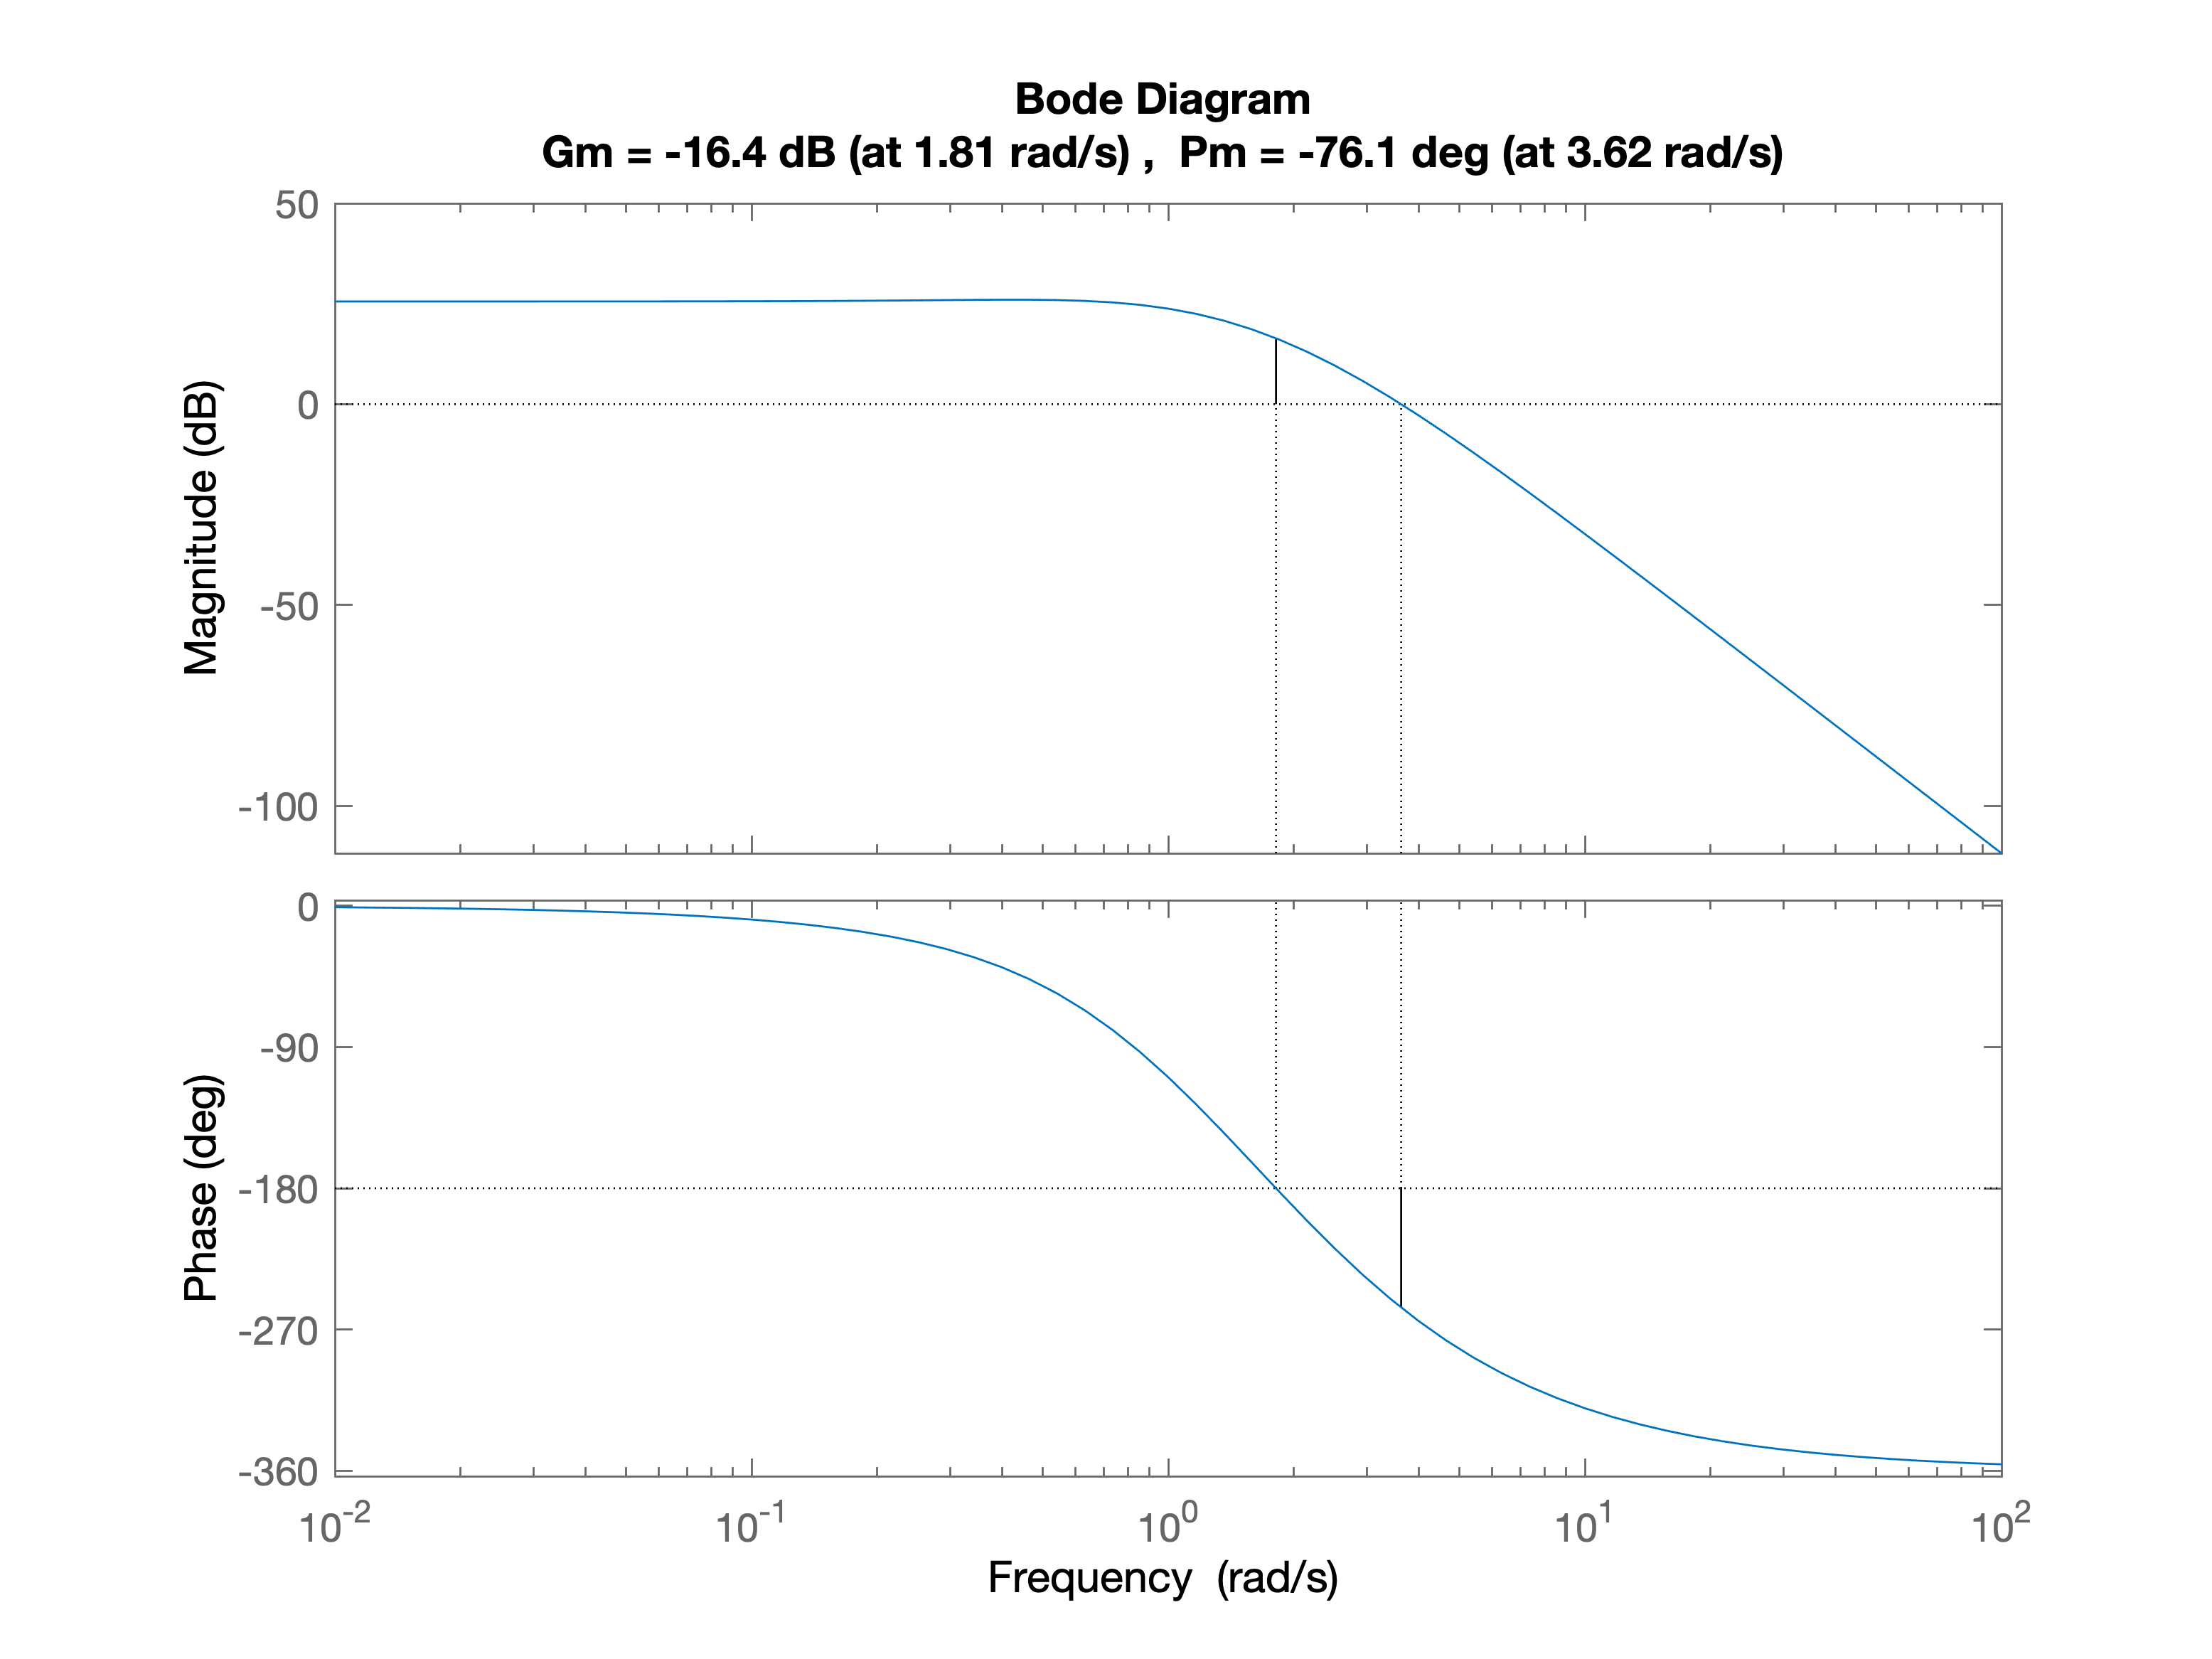
\includegraphics[width=12cm]{../Figure/Q1/a/margin.png}
\end{figure}
MATLAB bode digram and our calculation are exactly the same.
$$
\bar{\gamma} = 45 + 5 = 50^{\circ},\quad \phi_m = \bar{\gamma} - \gamma = 64.070^{\circ}
$$
$$
\sin(\phi_m) = \dfrac{1-\alpha}{1+\alpha} \to
\alpha = \dfrac{1-\sin(\phi_m) }{1+\sin(\phi_m) } = 0.0530
$$
$$
K_c = \dfrac{K}{\alpha} = \dfrac{5.1300}{0.0530} = 96.787
$$
$$
\left\vert G_1(j\omega_m) \right\vert = \sqrt{\alpha} = \left\vert KG(j\omega_m) \right\vert = 5.13 \dfrac{50\sqrt{\omega_m^2+0.5^2}}{\sqrt{\omega_m^2+1^2}\times(\sqrt{\omega_m^2 + 1.5^2})^3\times\sqrt{\omega_m^2 + 2^2}} = 0.230
$$
This equation solved with MATLAB and code has attacked (Q1\_a.m).
$$
\omega_m = 5.5226
$$
$$
\omega_m = \dfrac{1}{T\sqrt{\alpha}} \to
T = \dfrac{1}{\omega_m\sqrt{\alpha}} = \dfrac{1}{5.5226\sqrt{0.0530}} = 0.7865
$$
$$
G_c(s) = K_c \alpha \dfrac{Ts + 1}{\alpha T s + 1} = 96.787\dfrac{s + 1.2714}{s + 23.9880}
$$